\chapter{绪论}
\section{研究背景与意义}

请在此阐述研究背景、应用需求与理论意义。可从学科发展、行业应用或现有方法的不足等角度展开，并适当引用相关文献\cite{example-journal,example-conference}。

\section{研究内容与贡献}

本文的研究框架如图\ref{fig:ch1-framework}所示。请在此概述全文的研究内容、技术路线与主要贡献，可按条目列出。

\begin{figure}[t]
    \centering
    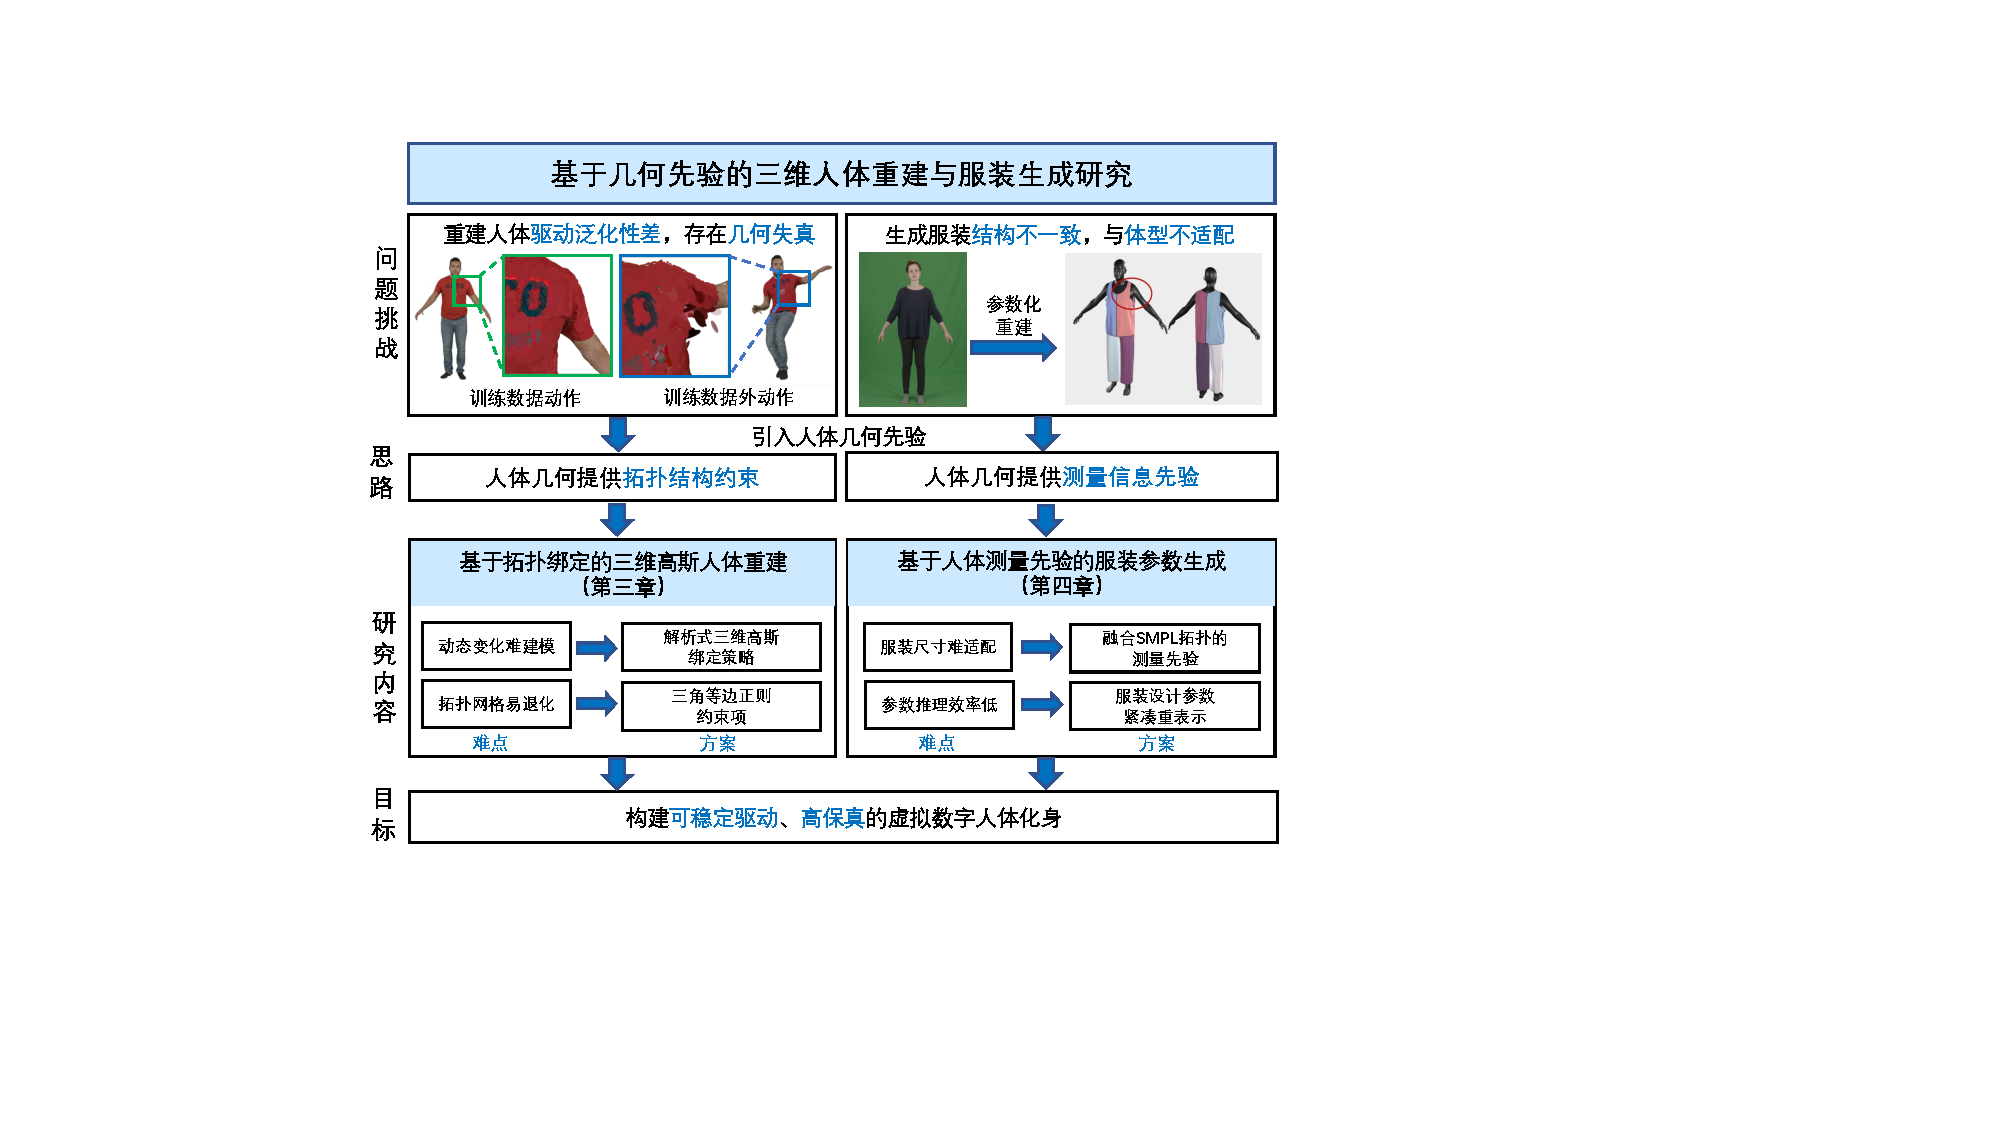
\includegraphics[width=\linewidth]{main/chapter1/figures/example-figure.pdf}
    \caption{示例插图：全文研究框架示意图（请替换为你的图片）}
    \label{fig:ch1-framework}
\end{figure}

本项工作的主要贡献包括：

（1）\textbf{贡献一}\enspace 请在此描述第一项主要贡献。

（2）\textbf{贡献二}\enspace 请在此描述第二项主要贡献。

（3）\textbf{贡献三}\enspace 请在此描述第三项主要贡献。

\section{论文结构安排}

本文共分为五章，各章内容安排如下。

第一章为绪论，介绍研究背景与意义、研究内容与贡献，以及论文结构安排。

第二章为相关研究综述，回顾与本课题相关的基础理论与代表性方法，并分析现有工作的不足。

第三章介绍所提出的核心方法，给出问题定义、方法设计与关键模块说明。

第四章给出实验设置、结果分析与讨论。

第五章为总结与展望，归纳全文工作并讨论未来研究方向。
